\documentclass[12pt]{article}
% Préambule commun à tous les documents extraits de « La Revue CAPES »
\usepackage[T1]{fontenc}
\usepackage[utf8]{inputenc}
\usepackage{lmodern}
\usepackage{amsmath,amssymb,amsthm,amsfonts,mathrsfs}
\usepackage{setspace}
\usepackage{listings}
\usepackage{pgfplots}
\pgfplotsset{compat=1.18}
\usepackage{longtable}
\usepackage{adjustbox}
\usepackage{lettrine}
\usepackage{tkz-tab}
\usepackage{changepage}
\usepackage{pdflscape}
\usepackage{graphicx}
\usepackage{tikz}
\usepackage{xcolor}
\usepackage[a4paper,top=2cm,bottom=2.5cm,left=2.5cm,right=2cm]{geometry}
\usepackage{fancyhdr}
\usepackage{draftwatermark}
\SetWatermarkText{La RevueCapes}
\SetWatermarkLightness{0.9}
\SetWatermarkScale{2}
\usepackage{hyperref}
\hypersetup{colorlinks=true,linkcolor=blue!50!black,urlcolor=blue!50!black}

\definecolor{revue}{RGB}{20,60,120}

\pagestyle{fancy}
\fancyhf{}
\renewcommand{\headrulewidth}{0.4pt}
\setlength{\headheight}{15pt}

% \entete{Matière}{Titre}{Type de document}
\newcommand{\entete}[3]{%
  \fancyhead[L]{\small\textsc{La Revue CAPES} -- #1}%
  \fancyhead[R]{\small #2}%
  \fancyfoot[C]{\thepage}%
  \thispagestyle{plain}%
  \begin{center}
    {\color{revue}\rule{\textwidth}{1.2pt}}\\[4pt]
    {\small\textsc{Concours directs CAP-CEG / CAPES -- Burkina Faso}}\\[6pt]
    {\LARGE\bfseries\color{revue} #2}\\[6pt]
    {\large\itshape #1 -- #3}\\[2pt]
    {\color{revue}\rule{\textwidth}{1.2pt}}
  \end{center}
  \vspace{0.5cm}%
}

% Encadré pour les remarques ajoutées dans les corrigés
\newcommand{\remarque}[1]{\par\medskip\noindent\fcolorbox{revue}{revue!6}{\parbox{\dimexpr\linewidth-2\fboxsep-2\fboxrule}{\textbf{\color{revue}Remarque.} #1}}\par\medskip}


\begin{document}
\entete{Mathématiques}{Corrigé détaillé -- Session 2016}{Correction}
\begin{spacing}{1.5}

\textbf{Exercice 1} \quad $(C)$ : $x(t)=\cos3t$, \ $y(t)=\sin2t$, \ $t\in\mathbb{R}$.

\textbf{1. Réduction de l'intervalle d'étude.}

\underline{Périodicité.} $x$ est $\frac{2\pi}{3}$-périodique et $y$ est $\pi$-périodique ; elles sont donc toutes deux $2\pi$-périodiques ($2\pi=3\times\frac{2\pi}3=2\times\pi$). Le point $M(t+2\pi)$ est égal à $M(t)$ : il suffit d'étudier $t\in[-\pi,\pi]$.

\underline{Parité.} $x(-t)=\cos(-3t)=\cos3t=x(t)$ et $y(-t)=\sin(-2t)=-\sin2t=-y(t)$. Le point $M(-t)$ est le symétrique de $M(t)$ par rapport à l'axe des abscisses $(Ox)$.

Il suffit donc d'étudier la courbe pour $t\in[0,\pi]$, puis de compléter par la symétrie d'axe $(Ox)$ : on obtient ainsi la courbe entière.

\textbf{2. Tableau des variations sur $[0,\pi]$.}

\underline{$x'(t)=-3\sin3t$.} Sur $[0,\pi]$, $3t\in[0,3\pi]$ : $\sin3t\ge0$ pour $t\in[0,\frac\pi3]\cup[\frac{2\pi}3,\pi]$ et $\sin3t\le0$ pour $t\in[\frac\pi3,\frac{2\pi}3]$. Donc $x'\le0$ sur $[0,\frac\pi3]$ et sur $[\frac{2\pi}3,\pi]$, $x'\ge0$ sur $[\frac\pi3,\frac{2\pi}3]$ ; $x'$ s'annule en $0,\frac\pi3,\frac{2\pi}3,\pi$.

\underline{$y'(t)=2\cos2t$.} Sur $[0,\pi]$, $2t\in[0,2\pi]$ : $y'\ge0$ sur $[0,\frac\pi4]$ et sur $[\frac{3\pi}4,\pi]$, $y'\le0$ sur $[\frac\pi4,\frac{3\pi}4]$ ; $y'$ s'annule en $\frac\pi4$ et $\frac{3\pi}4$.

\underline{Valeurs utiles.}
\begin{center}
\begin{tabular}{|c|c|c|c|c|c|c|}
\hline
$t$ & $0$ & $\frac\pi4$ & $\frac\pi3$ & $\frac{2\pi}3$ & $\frac{3\pi}4$ & $\pi$\\
\hline
$x(t)=\cos3t$ & $1$ & $-\frac{\sqrt2}2$ & $-1$ & $1$ & $\frac{\sqrt2}2$ & $-1$\\
\hline
$y(t)=\sin2t$ & $0$ & $1$ & $\frac{\sqrt3}2$ & $-\frac{\sqrt3}2$ & $-1$ & $0$\\
\hline
\end{tabular}
\end{center}

\begin{center}
\resizebox{\textwidth}{!}{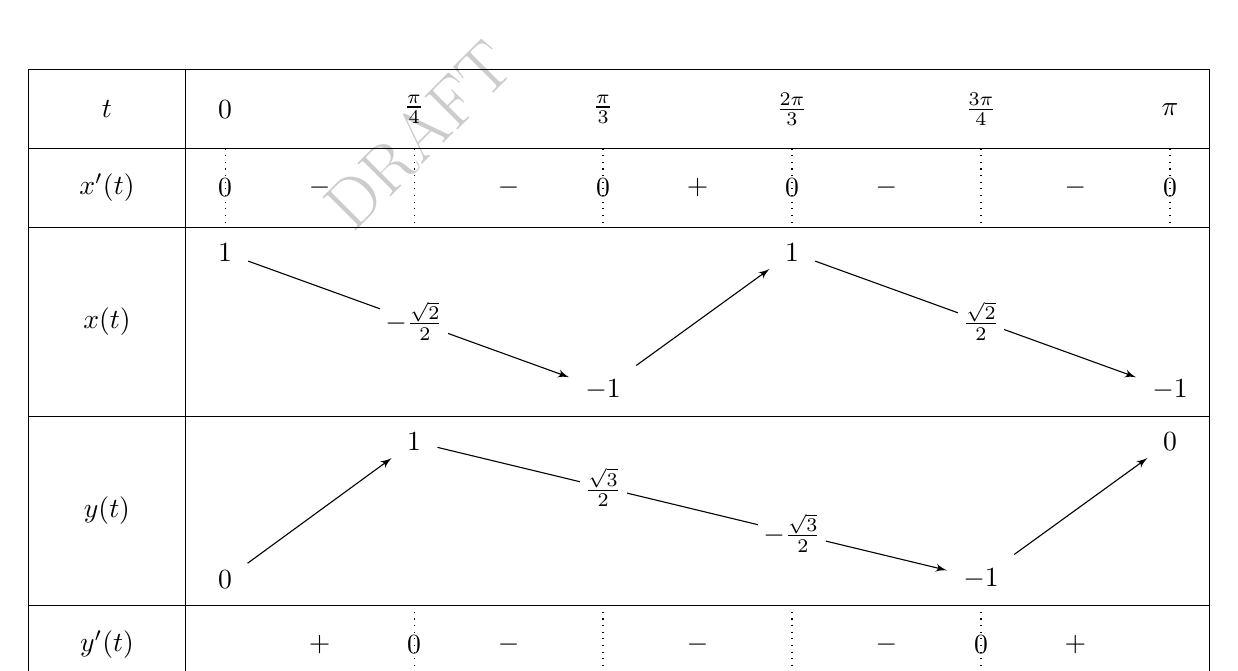
\begin{tikzpicture}
\tkzTabInit[lgt=2, espcl=2.4]{$t$ /1, $x'(t)$ /1, $x(t)$ /2.4, $y(t)$ /2.4, $y'(t)$ /1}{$0$, $\frac{\pi}{4}$, $\frac{\pi}{3}$, $\frac{2\pi}{3}$, $\frac{3\pi}{4}$, $\pi$}
\tkzTabLine{z, -, t, -, z, +, z, -, t, -, z}
\tkzTabVar{+/$1$, R/, -/$-1$, +/$1$, R/, -/$-1$}
\tkzTabIma{1}{3}{2}{$-\frac{\sqrt2}{2}$}
\tkzTabIma{4}{6}{5}{$\frac{\sqrt2}{2}$}
\tkzTabVar{-/$0$, +/$1$, R/, R/, -/$-1$, +/$0$}
\tkzTabIma{2}{5}{3}{$\frac{\sqrt3}{2}$}
\tkzTabIma{2}{5}{4}{$-\frac{\sqrt3}{2}$}
\tkzTabLine{, +, z, -, t, -, t, -, z, +, }
\end{tikzpicture}}
\end{center}

\underline{Tangentes remarquables} (le vecteur $(x'(t),y'(t))$ ne s'annule jamais car $x'$ et $y'$ n'ont pas de zéro commun sur $[0,\pi]$) :
\begin{itemize}
\item tangentes \emph{verticales} ($x'=0$) en $t=0$ : $(1,0)$ ; $t=\frac\pi3$ : $\big(-1,\frac{\sqrt3}2\big)$ ; $t=\frac{2\pi}3$ : $\big(1,-\frac{\sqrt3}2\big)$ ; $t=\pi$ : $(-1,0)$ ;
\item tangentes \emph{horizontales} ($y'=0$) en $t=\frac\pi4$ : $\big(-\frac{\sqrt2}2,1\big)$ ; $t=\frac{3\pi}4$ : $\big(\frac{\sqrt2}2,-1\big)$.
\end{itemize}

\textbf{3. Tracé de $(C)$.} On trace l'arc correspondant à $t\in[0,\pi]$ (en trait plein) puis son symétrique par rapport à $(Ox)$ (en pointillés). La courbe (courbe de Lissajous) est inscrite dans le carré $[-1,1]^2$.
\begin{center}
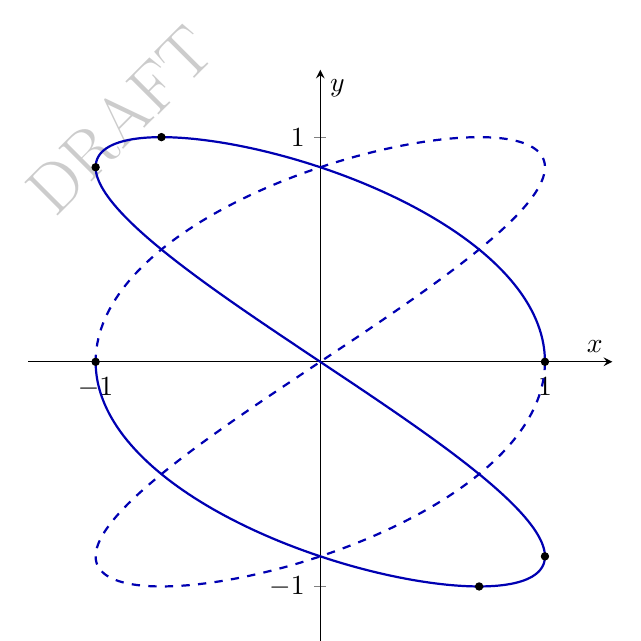
\begin{tikzpicture}
\begin{axis}[axis lines=middle, xlabel=$x$, ylabel=$y$, xmin=-1.3, xmax=1.3, ymin=-1.3, ymax=1.3, width=9cm, height=9cm, samples=300, domain=0:3.14159, xtick={-1,1}, ytick={-1,1}]
\addplot[blue!70!black, thick, variable=\t, parametric] ({cos(deg(3*t))},{sin(deg(2*t))});
\addplot[blue!70!black, thick, dashed, variable=\t, parametric] ({cos(deg(3*t))},{-sin(deg(2*t))});
\addplot[only marks, mark=*, mark size=1.3pt] coordinates {(1,0) (-0.7071,1) (-1,0.866) (1,-0.866) (0.7071,-1) (-1,0)};
\end{axis}
\end{tikzpicture}
\end{center}

\medskip\textbf{Exercice 2} \quad $x\,\nabla\,y\iff xe^y=ye^x$.

\textbf{1. Réflexivité.} Pour tout réel $x$, $xe^x=xe^x$, donc $x\,\nabla\,x$.

\textbf{2. Symétrie.} Si $x\,\nabla\,y$, alors $xe^y=ye^x$, c'est-à-dire $ye^x=xe^y$, donc $y\,\nabla\,x$.

\textbf{3.} Si $x\,\nabla\,y$ et $y\,\nabla\,z$ : $xe^y=ye^x$ (1) et $ye^z=ze^y$ (2). En multipliant membre à membre :
\[
xe^y\cdot ye^z=ye^x\cdot ze^y\quad\Longrightarrow\quad xy\,e^z=yz\,e^x\qquad(\text{après division par } e^y>0).
\]

\textbf{4. Transitivité ; relation d'équivalence.} Supposons $x\,\nabla\,y$ et $y\,\nabla\,z$.
\begin{itemize}
\item Si $y\neq0$ : en divisant l'égalité de la question 3 par $y$, $xe^z=ze^x$, donc $x\,\nabla\,z$.
\item Si $y=0$ : $x\,\nabla\,0$ s'écrit $xe^0=0\cdot e^x$, soit $x=0$ ; de même $0\,\nabla\,z$ donne $z=0$. Alors $x=z=0$ et $x\,\nabla\,z$ (réflexivité).
\end{itemize}
La relation $\nabla$ est réflexive, symétrique et transitive : c'est une \textbf{relation d'équivalence}.

\remarque{On a $x\,\nabla\,y\iff\varphi(x)=\varphi(y)$ avec $\varphi(t)=te^{-t}$ ; une relation de la forme « avoir la même image par une fonction » est toujours une relation d'équivalence.}

\medskip\textbf{Exercice 3}

\textbf{1.a) Inversibilité de $A=\begin{pmatrix}1&0&a\\0&a&1\\a&1&0\end{pmatrix}$.} En développant suivant la première ligne :
\[
\det A=1\cdot\begin{vmatrix}a&1\\1&0\end{vmatrix}-0+a\begin{vmatrix}0&a\\a&1\end{vmatrix}=(0-1)+a(0-a^2)=-(1+a^3).
\]
Or $1+a^3=(1+a)(1-a+a^2)$ et $1-a+a^2$ a un discriminant $1-4<0$, donc ne s'annule jamais. Ainsi $\det A=0\iff a=-1$ :
\[
\boxed{A\text{ est inversible}\iff a\neq-1}.
\]

\textbf{1.b) Inverse.} Les cofacteurs $C_{ij}=(-1)^{i+j}\Delta_{ij}$ sont :
\[
\operatorname{com}(A)=\begin{pmatrix}-1&a&-a^2\\a&-a^2&-1\\-a^2&-1&a\end{pmatrix}
\]
(par exemple $C_{11}=a\cdot0-1\cdot1=-1$, $C_{12}=-(0\cdot0-1\cdot a)=a$, $C_{13}=0\cdot1-a\cdot a=-a^2$). Cette matrice est symétrique (comme $A$), donc ${}^t\operatorname{com}(A)=\operatorname{com}(A)$ et, pour $a\neq-1$ :
\[
A^{-1}=\frac{1}{\det A}\,{}^t\operatorname{com}(A)=\boxed{\frac{1}{1+a^3}\begin{pmatrix}1&-a&a^2\\-a&a^2&1\\a^2&1&-a\end{pmatrix}}.
\]
(Vérification de la première colonne de $AA^{-1}$ : $\frac{1}{1+a^3}(1+a^3,\ -a^2+a^2,\ a-a)=(1,0,0)$.)

\textbf{2.a) Transposée de $B=\begin{pmatrix}3&0&-1\\2&4&2\\-1&0&3\end{pmatrix}$.}
\[
{}^tB=\begin{pmatrix}3&2&-1\\0&4&0\\-1&2&3\end{pmatrix}.
\]

\textbf{2.b) Polynôme caractéristique.} En développant suivant la deuxième colonne (un seul coefficient non nul) :
\[
P_B(x)=\det(B-xI_3)=\begin{vmatrix}3-x&0&-1\\2&4-x&2\\-1&0&3-x\end{vmatrix}=(4-x)\begin{vmatrix}3-x&-1\\-1&3-x\end{vmatrix}=(4-x)\big[(3-x)^2-1\big],
\]
\[
\boxed{P_B(x)=(4-x)(2-x)(4-x)=(2-x)(4-x)^2}.
\]

\textbf{2.c) Valeurs propres, diagonalisation.} Les racines de $P_B$ sont $2$ (simple) et $4$ (double) : ce sont les valeurs propres de $B$.

\underline{$E_2=\ker(B-2I)$} : $\begin{cases}x-z=0\\2x+2y+2z=0\\-x+z=0\end{cases}\iff\begin{cases}z=x\\y=-2x\end{cases}$, donc $E_2=\operatorname{Vect}\big((1,-2,1)\big)$.

\underline{$E_4=\ker(B-4I)$} : $\begin{cases}-x-z=0\\2x+2z=0\\-x-z=0\end{cases}\iff z=-x$, $y$ quelconque. Donc $(x,y,z)=y(0,1,0)+x(1,0,-1)$ et $E_4=\operatorname{Vect}\big((0,1,0),(-1,0,1)\big)$, de dimension $2$.

$\dim E_2+\dim E_4=1+2=3$ : chaque sous-espace propre a pour dimension la multiplicité de la valeur propre, \textbf{$B$ est diagonalisable}.
\[
D=\begin{pmatrix}2&0&0\\0&4&0\\0&0&4\end{pmatrix},\qquad P=\begin{pmatrix}1&0&-1\\-2&1&0\\1&0&1\end{pmatrix},\qquad B=PDP^{-1}.
\]
\underline{Inverse de $P$.} En développant suivant la deuxième colonne, $\det P=1\cdot\begin{vmatrix}1&-1\\1&1\end{vmatrix}=2$, et par la comatrice :
\[
P^{-1}=\frac12\begin{pmatrix}1&0&1\\2&2&2\\-1&0&1\end{pmatrix}.
\]

\textbf{2.d) Calcul de $B^n$.} Par récurrence, $B^n=PD^nP^{-1}$ avec $D^n=\operatorname{diag}(2^n,4^n,4^n)$ :
\[
PD^n=\begin{pmatrix}2^n&0&-4^n\\-2\cdot2^n&4^n&0\\2^n&0&4^n\end{pmatrix},\qquad
\boxed{B^n=\frac12\begin{pmatrix}2^n+4^n&0&2^n-4^n\\2\cdot4^n-2\cdot2^n&2\cdot4^n&2\cdot4^n-2\cdot2^n\\2^n-4^n&0&2^n+4^n\end{pmatrix}}
\]
soit $B^n=\begin{pmatrix}\frac{2^n+4^n}{2}&0&\frac{2^n-4^n}{2}\\4^n-2^n&4^n&4^n-2^n\\\frac{2^n-4^n}{2}&0&\frac{2^n+4^n}{2}\end{pmatrix}$. (Pour $n=1$ on retrouve $B$.)

\medskip\textbf{Exercice 4} \quad $f(x,y)=\dfrac{xy^3}{x^4+y^2}$ si $(x,y)\neq(0,0)$, $f(0,0)=0$.

\textbf{1. Domaine de définition.} $x^4+y^2=0\iff x=y=0$. L'expression $\frac{xy^3}{x^4+y^2}$ est donc définie sur $\mathbb{R}^2\setminus\{(0,0)\}$, et $f$ étant aussi définie en $(0,0)$ par $f(0,0)=0$ : $\boxed{D_f=\mathbb{R}^2}$.

\textbf{2. Inégalité.} Pour tous réels $a,b$ : $a^2+b^2-2ab=(a-b)^2\ge0$, donc $a^2+b^2\ge2ab$. Avec $a=x^2$ et $b=y$ : $x^4+y^2\ge2x^2y$ (et, avec $b=|y|$, $x^4+y^2\ge2x^2|y|$).

\textbf{3. Continuité en $(0,0)$.} Pour $(x,y)\neq(0,0)$, comme $x^4+y^2\ge y^2$ :
\[
|f(x,y)|=|x|\,|y|\cdot\frac{y^2}{x^4+y^2}\le|x|\,|y|\xrightarrow[(x,y)\to(0,0)]{}0 .
\]
Donc $\lim\limits_{(0,0)}f=0=f(0,0)$ : $f$ est continue en $(0,0)$ (et sur $\mathbb{R}^2$, car c'est une fraction rationnelle ailleurs).

\remarque{Avec l'inégalité de la question 2, on peut aussi écrire $|f(x,y)|=\frac{|x|y^2\,|y|}{x^4+y^2}\le\frac{|x|y^2|y|}{2x^2|y|}=\frac{y^2}{2|x|}$ pour $xy\neq0$, mais ce majorant ne tend pas vers $0$ (prendre $y^2=x$) : il faut donc utiliser la majoration ci-dessus.}

\textbf{4. Dérivées partielles et continuité.}

\underline{Pour $(x,y)\neq(0,0)$} (dérivée d'un quotient) :
\[
\frac{\partial f}{\partial x}=\frac{y^3(x^4+y^2)-xy^3\cdot4x^3}{(x^4+y^2)^2}=\frac{y^3(y^2-3x^4)}{(x^4+y^2)^2},\qquad
\frac{\partial f}{\partial y}=\frac{3xy^2(x^4+y^2)-xy^3\cdot2y}{(x^4+y^2)^2}=\frac{xy^2(3x^4+y^2)}{(x^4+y^2)^2}.
\]
\underline{En $(0,0)$} (par définition) : $f(x,0)=0$ et $f(0,y)=0$ pour tous $x,y$, donc
\[
\frac{\partial f}{\partial x}(0,0)=\lim_{h\to0}\frac{f(h,0)-0}{h}=0,\qquad\frac{\partial f}{\partial y}(0,0)=\lim_{k\to0}\frac{f(0,k)-0}{k}=0 .
\]
\underline{Continuité en $(0,0)$.} Il faut une majoration valable dans toutes les directions (et pas seulement quand $y\to0$). Comme $|y^2-3x^4|\le3(x^4+y^2)$ et $y^2\le x^4+y^2$ :
\[
\Big|\frac{\partial f}{\partial x}(x,y)\Big|\le\frac{|y|^3\cdot3(x^4+y^2)}{(x^4+y^2)^2}=\frac{3|y|\,y^2}{x^4+y^2}\le3|y|\to0,
\]
\[
\Big|\frac{\partial f}{\partial y}(x,y)\Big|\le\frac{|x|y^2\cdot3(x^4+y^2)}{(x^4+y^2)^2}=\frac{3|x|\,y^2}{x^4+y^2}\le3|x|\to0 .
\]
Les dérivées partielles tendent vers $0$, leur valeur en $(0,0)$ : elles sont continues en $(0,0)$, et sur $\mathbb{R}^2\setminus\{(0,0)\}$ (fractions rationnelles). \textbf{$f$ est donc de classe $C^1$ sur $\mathbb{R}^2$.}

\end{spacing}
\end{document}
